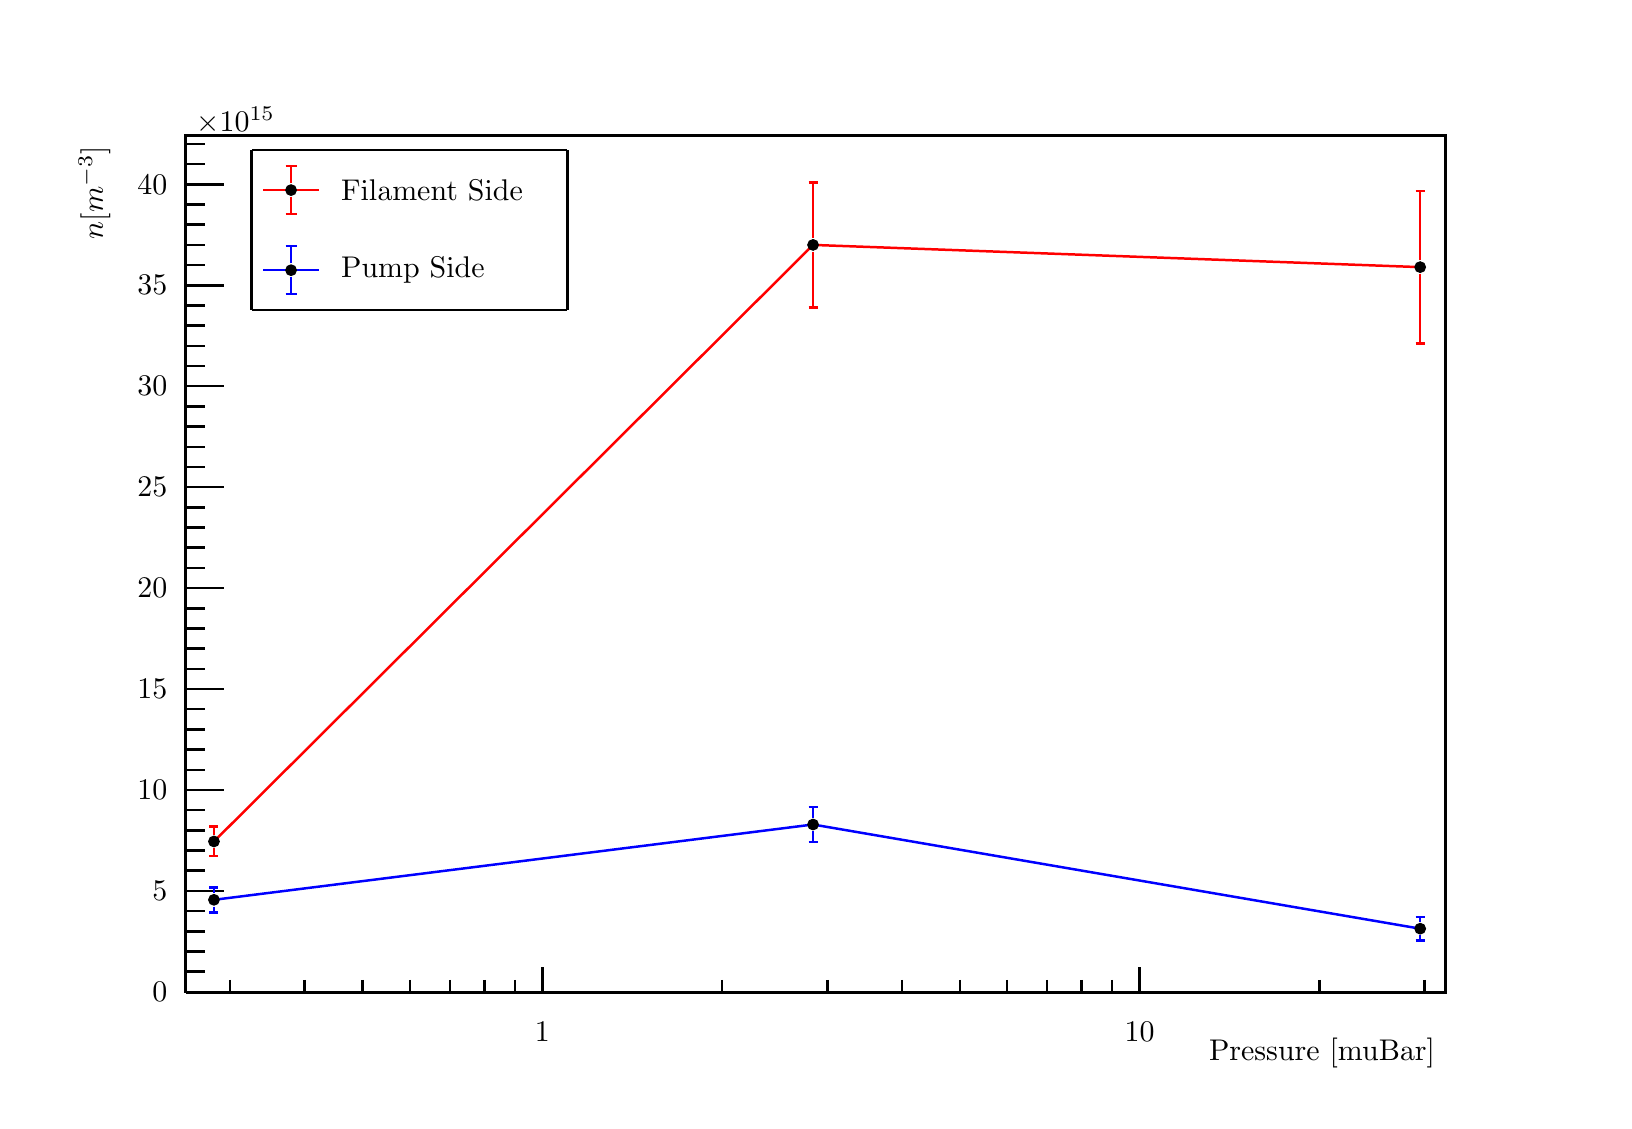
\begin{tikzpicture}
\pgfdeclareplotmark{cross} {
\pgfpathmoveto{\pgfpoint{-0.3\pgfplotmarksize}{\pgfplotmarksize}}
\pgfpathlineto{\pgfpoint{+0.3\pgfplotmarksize}{\pgfplotmarksize}}
\pgfpathlineto{\pgfpoint{+0.3\pgfplotmarksize}{0.3\pgfplotmarksize}}
\pgfpathlineto{\pgfpoint{+1\pgfplotmarksize}{0.3\pgfplotmarksize}}
\pgfpathlineto{\pgfpoint{+1\pgfplotmarksize}{-0.3\pgfplotmarksize}}
\pgfpathlineto{\pgfpoint{+0.3\pgfplotmarksize}{-0.3\pgfplotmarksize}}
\pgfpathlineto{\pgfpoint{+0.3\pgfplotmarksize}{-1.\pgfplotmarksize}}
\pgfpathlineto{\pgfpoint{-0.3\pgfplotmarksize}{-1.\pgfplotmarksize}}
\pgfpathlineto{\pgfpoint{-0.3\pgfplotmarksize}{-0.3\pgfplotmarksize}}
\pgfpathlineto{\pgfpoint{-1.\pgfplotmarksize}{-0.3\pgfplotmarksize}}
\pgfpathlineto{\pgfpoint{-1.\pgfplotmarksize}{0.3\pgfplotmarksize}}
\pgfpathlineto{\pgfpoint{-0.3\pgfplotmarksize}{0.3\pgfplotmarksize}}
\pgfpathclose
\pgfusepathqstroke
}
\pgfdeclareplotmark{cross*} {
\pgfpathmoveto{\pgfpoint{-0.3\pgfplotmarksize}{\pgfplotmarksize}}
\pgfpathlineto{\pgfpoint{+0.3\pgfplotmarksize}{\pgfplotmarksize}}
\pgfpathlineto{\pgfpoint{+0.3\pgfplotmarksize}{0.3\pgfplotmarksize}}
\pgfpathlineto{\pgfpoint{+1\pgfplotmarksize}{0.3\pgfplotmarksize}}
\pgfpathlineto{\pgfpoint{+1\pgfplotmarksize}{-0.3\pgfplotmarksize}}
\pgfpathlineto{\pgfpoint{+0.3\pgfplotmarksize}{-0.3\pgfplotmarksize}}
\pgfpathlineto{\pgfpoint{+0.3\pgfplotmarksize}{-1.\pgfplotmarksize}}
\pgfpathlineto{\pgfpoint{-0.3\pgfplotmarksize}{-1.\pgfplotmarksize}}
\pgfpathlineto{\pgfpoint{-0.3\pgfplotmarksize}{-0.3\pgfplotmarksize}}
\pgfpathlineto{\pgfpoint{-1.\pgfplotmarksize}{-0.3\pgfplotmarksize}}
\pgfpathlineto{\pgfpoint{-1.\pgfplotmarksize}{0.3\pgfplotmarksize}}
\pgfpathlineto{\pgfpoint{-0.3\pgfplotmarksize}{0.3\pgfplotmarksize}}
\pgfpathclose
\pgfusepathqfillstroke
}
\pgfdeclareplotmark{newstar} {
\pgfpathmoveto{\pgfqpoint{0pt}{\pgfplotmarksize}}
\pgfpathlineto{\pgfqpointpolar{44}{0.5\pgfplotmarksize}}
\pgfpathlineto{\pgfqpointpolar{18}{\pgfplotmarksize}}
\pgfpathlineto{\pgfqpointpolar{-20}{0.5\pgfplotmarksize}}
\pgfpathlineto{\pgfqpointpolar{-54}{\pgfplotmarksize}}
\pgfpathlineto{\pgfqpointpolar{-90}{0.5\pgfplotmarksize}}
\pgfpathlineto{\pgfqpointpolar{234}{\pgfplotmarksize}}
\pgfpathlineto{\pgfqpointpolar{198}{0.5\pgfplotmarksize}}
\pgfpathlineto{\pgfqpointpolar{162}{\pgfplotmarksize}}
\pgfpathlineto{\pgfqpointpolar{134}{0.5\pgfplotmarksize}}
\pgfpathclose
\pgfusepathqstroke
}
\pgfdeclareplotmark{newstar*} {
\pgfpathmoveto{\pgfqpoint{0pt}{\pgfplotmarksize}}
\pgfpathlineto{\pgfqpointpolar{44}{0.5\pgfplotmarksize}}
\pgfpathlineto{\pgfqpointpolar{18}{\pgfplotmarksize}}
\pgfpathlineto{\pgfqpointpolar{-20}{0.5\pgfplotmarksize}}
\pgfpathlineto{\pgfqpointpolar{-54}{\pgfplotmarksize}}
\pgfpathlineto{\pgfqpointpolar{-90}{0.5\pgfplotmarksize}}
\pgfpathlineto{\pgfqpointpolar{234}{\pgfplotmarksize}}
\pgfpathlineto{\pgfqpointpolar{198}{0.5\pgfplotmarksize}}
\pgfpathlineto{\pgfqpointpolar{162}{\pgfplotmarksize}}
\pgfpathlineto{\pgfqpointpolar{134}{0.5\pgfplotmarksize}}
\pgfpathclose
\pgfusepathqfillstroke
}
\definecolor{c}{rgb}{1,1,1};
\draw [color=c, fill=c] (0,0) rectangle (20,13.6103);
\draw [color=c, fill=c] (2,1.36103) rectangle (18,12.2493);
\definecolor{c}{rgb}{0,0,0};
\draw [c,line width=0.9] (2,1.36103) -- (2,12.2493) -- (18,12.2493) -- (18,1.36103) -- (2,1.36103);
\definecolor{c}{rgb}{1,1,1};
\draw [color=c, fill=c] (2,1.36103) rectangle (18,12.2493);
\definecolor{c}{rgb}{0,0,0};
\draw [c,line width=0.9] (2,1.36103) -- (2,12.2493) -- (18,12.2493) -- (18,1.36103) -- (2,1.36103);
\draw [c,line width=0.9] (2,1.36103) -- (18,1.36103);
\draw [c,line width=0.9] (2.56262,1.52436) -- (2.56262,1.36103);
\draw [c,line width=0.9] (3.51031,1.52436) -- (3.51031,1.36103);
\draw [c,line width=0.9] (4.2454,1.52436) -- (4.2454,1.36103);
\draw [c,line width=0.9] (4.84601,1.52436) -- (4.84601,1.36103);
\draw [c,line width=0.9] (5.35381,1.52436) -- (5.35381,1.36103);
\draw [c,line width=0.9] (5.79369,1.52436) -- (5.79369,1.36103);
\draw [c,line width=0.9] (6.1817,1.52436) -- (6.1817,1.36103);
\draw [c,line width=0.9] (6.52878,1.68768) -- (6.52878,1.36103);
\draw [anchor=base] (6.52878,0.745165) node[scale=1.08185, color=c, rotate=0]{1};
\draw [c,line width=0.9] (8.81216,1.52436) -- (8.81216,1.36103);
\draw [c,line width=0.9] (10.1479,1.52436) -- (10.1479,1.36103);
\draw [c,line width=0.9] (11.0955,1.52436) -- (11.0955,1.36103);
\draw [c,line width=0.9] (11.8306,1.52436) -- (11.8306,1.36103);
\draw [c,line width=0.9] (12.4312,1.52436) -- (12.4312,1.36103);
\draw [c,line width=0.9] (12.939,1.52436) -- (12.939,1.36103);
\draw [c,line width=0.9] (13.3789,1.52436) -- (13.3789,1.36103);
\draw [c,line width=0.9] (13.7669,1.52436) -- (13.7669,1.36103);
\draw [c,line width=0.9] (14.114,1.68768) -- (14.114,1.36103);
\draw [anchor=base] (14.114,0.745165) node[scale=1.08185, color=c, rotate=0]{10};
\draw [c,line width=0.9] (16.3974,1.52436) -- (16.3974,1.36103);
\draw [c,line width=0.9] (17.7331,1.52436) -- (17.7331,1.36103);
\draw [anchor= east] (18,0.598854) node[scale=1.08185, color=c, rotate=0]{Pressure [muBar]};
\draw [c,line width=0.9] (2,1.36103) -- (2,12.2493);
\draw [c,line width=0.9] (2.48,1.37206) -- (2,1.37206);
\draw [c,line width=0.9] (2.24,1.62844) -- (2,1.62844);
\draw [c,line width=0.9] (2.24,1.88482) -- (2,1.88482);
\draw [c,line width=0.9] (2.24,2.1412) -- (2,2.1412);
\draw [c,line width=0.9] (2.24,2.39759) -- (2,2.39759);
\draw [c,line width=0.9] (2.48,2.65397) -- (2,2.65397);
\draw [c,line width=0.9] (2.24,2.91035) -- (2,2.91035);
\draw [c,line width=0.9] (2.24,3.16673) -- (2,3.16673);
\draw [c,line width=0.9] (2.24,3.42311) -- (2,3.42311);
\draw [c,line width=0.9] (2.24,3.67949) -- (2,3.67949);
\draw [c,line width=0.9] (2.48,3.93587) -- (2,3.93587);
\draw [c,line width=0.9] (2.24,4.19225) -- (2,4.19225);
\draw [c,line width=0.9] (2.24,4.44864) -- (2,4.44864);
\draw [c,line width=0.9] (2.24,4.70502) -- (2,4.70502);
\draw [c,line width=0.9] (2.24,4.9614) -- (2,4.9614);
\draw [c,line width=0.9] (2.48,5.21778) -- (2,5.21778);
\draw [c,line width=0.9] (2.24,5.47416) -- (2,5.47416);
\draw [c,line width=0.9] (2.24,5.73054) -- (2,5.73054);
\draw [c,line width=0.9] (2.24,5.98692) -- (2,5.98692);
\draw [c,line width=0.9] (2.24,6.2433) -- (2,6.2433);
\draw [c,line width=0.9] (2.48,6.49969) -- (2,6.49969);
\draw [c,line width=0.9] (2.24,6.75607) -- (2,6.75607);
\draw [c,line width=0.9] (2.24,7.01245) -- (2,7.01245);
\draw [c,line width=0.9] (2.24,7.26883) -- (2,7.26883);
\draw [c,line width=0.9] (2.24,7.52521) -- (2,7.52521);
\draw [c,line width=0.9] (2.48,7.78159) -- (2,7.78159);
\draw [c,line width=0.9] (2.24,8.03797) -- (2,8.03797);
\draw [c,line width=0.9] (2.24,8.29435) -- (2,8.29435);
\draw [c,line width=0.9] (2.24,8.55074) -- (2,8.55074);
\draw [c,line width=0.9] (2.24,8.80712) -- (2,8.80712);
\draw [c,line width=0.9] (2.48,9.0635) -- (2,9.0635);
\draw [c,line width=0.9] (2.24,9.31988) -- (2,9.31988);
\draw [c,line width=0.9] (2.24,9.57626) -- (2,9.57626);
\draw [c,line width=0.9] (2.24,9.83264) -- (2,9.83264);
\draw [c,line width=0.9] (2.24,10.089) -- (2,10.089);
\draw [c,line width=0.9] (2.48,10.3454) -- (2,10.3454);
\draw [c,line width=0.9] (2.24,10.6018) -- (2,10.6018);
\draw [c,line width=0.9] (2.24,10.8582) -- (2,10.8582);
\draw [c,line width=0.9] (2.24,11.1145) -- (2,11.1145);
\draw [c,line width=0.9] (2.24,11.3709) -- (2,11.3709);
\draw [c,line width=0.9] (2.48,11.6273) -- (2,11.6273);
\draw [c,line width=0.9] (2.48,1.37206) -- (2,1.37206);
\draw [c,line width=0.9] (2.48,11.6273) -- (2,11.6273);
\draw [c,line width=0.9] (2.24,11.8837) -- (2,11.8837);
\draw [c,line width=0.9] (2.24,12.1401) -- (2,12.1401);
\draw [anchor= east] (1.9,1.37206) node[scale=1.08185, color=c, rotate=0]{0};
\draw [anchor= east] (1.9,2.65397) node[scale=1.08185, color=c, rotate=0]{5};
\draw [anchor= east] (1.9,3.93587) node[scale=1.08185, color=c, rotate=0]{10};
\draw [anchor= east] (1.9,5.21778) node[scale=1.08185, color=c, rotate=0]{15};
\draw [anchor= east] (1.9,6.49969) node[scale=1.08185, color=c, rotate=0]{20};
\draw [anchor= east] (1.9,7.78159) node[scale=1.08185, color=c, rotate=0]{25};
\draw [anchor= east] (1.9,9.0635) node[scale=1.08185, color=c, rotate=0]{30};
\draw [anchor= east] (1.9,10.3454) node[scale=1.08185, color=c, rotate=0]{35};
\draw [anchor= east] (1.9,11.6273) node[scale=1.08185, color=c, rotate=0]{40};
\draw [anchor=base west] (2,12.2969) node[scale=1.08185, color=c, rotate=0]{$\times10^{15}$};
\draw [anchor= east] (0.841547,12.2493) node[scale=1.08185, color=c, rotate=90]{$n [m^{-3}]$};
\definecolor{c}{rgb}{1,0,0};
\draw [c,line width=0.9] (2.35878,3.2821) -- (9.9673,10.8582) -- (17.6777,10.5761);
\definecolor{c}{rgb}{0,0,0};
\foreach \P in {(2.35878,3.2821), (9.9673,10.8582), (17.6777,10.5761)}{\draw[mark options={color=c,fill=c},mark size=1.921922pt,mark=*] plot coordinates {\P};}
\definecolor{c}{rgb}{1,0,0};
\draw [c,line width=0.9] (2.35878,3.36806) -- (2.35878,3.46952);
\draw [c,line width=0.9] (2.30148,3.46952) -- (2.41609,3.46952);
\draw [c,line width=0.9] (2.35878,3.19614) -- (2.35878,3.09469);
\draw [c,line width=0.9] (2.30148,3.09469) -- (2.41609,3.09469);
\draw [c,line width=0.9] (9.9673,10.9441) -- (9.9673,11.6504);
\draw [c,line width=0.9] (9.91,11.6504) -- (10.0246,11.6504);
\draw [c,line width=0.9] (9.9673,10.7722) -- (9.9673,10.0659);
\draw [c,line width=0.9] (9.91,10.0659) -- (10.0246,10.0659);
\draw [c,line width=0.9] (17.6777,10.6621) -- (17.6777,11.5453);
\draw [c,line width=0.9] (17.6204,11.5453) -- (17.735,11.5453);
\draw [c,line width=0.9] (17.6777,10.4902) -- (17.6777,9.60703);
\draw [c,line width=0.9] (17.6204,9.60703) -- (17.735,9.60703);
\definecolor{c}{rgb}{0,0,1};
\draw [c,line width=0.9] (2.35878,2.62712) -- (2.35878,2.69986);
\draw [c,line width=0.9] (2.30148,2.69986) -- (2.41609,2.69986);
\draw [c,line width=0.9] (2.35878,2.4552) -- (2.35878,2.38246);
\draw [c,line width=0.9] (2.30148,2.38246) -- (2.41609,2.38246);
\draw [c,line width=0.9] (9.9673,3.58342) -- (9.9673,3.71949);
\draw [c,line width=0.9] (9.91,3.71949) -- (10.0246,3.71949);
\draw [c,line width=0.9] (9.9673,3.4115) -- (9.9673,3.27544);
\draw [c,line width=0.9] (9.91,3.27544) -- (10.0246,3.27544);
\draw [c,line width=0.9] (17.6777,2.26049) -- (17.6777,2.324);
\draw [c,line width=0.9] (17.6204,2.324) -- (17.735,2.324);
\draw [c,line width=0.9] (17.6777,2.08857) -- (17.6777,2.02506);
\draw [c,line width=0.9] (17.6204,2.02506) -- (17.735,2.02506);
\draw [c,line width=0.9] (2.35878,2.54116) -- (9.9673,3.49746) -- (17.6777,2.17453);
\definecolor{c}{rgb}{0,0,0};
\foreach \P in {(2.35878,2.54116), (9.9673,3.49746), (17.6777,2.17453)}{\draw[mark options={color=c,fill=c},mark size=1.921922pt,mark=*] plot coordinates {\P};}
\definecolor{c}{rgb}{1,1,1};
\draw [color=c, fill=c] (2.83668,10.0287) rectangle (6.84814,12.063);
\definecolor{c}{rgb}{0,0,0};
\draw [c,line width=0.9] (2.83668,10.0287) -- (6.84814,10.0287);
\draw [c,line width=0.9] (6.84814,10.0287) -- (6.84814,12.063);
\draw [c,line width=0.9] (6.84814,12.063) -- (2.83668,12.063);
\draw [c,line width=0.9] (2.83668,12.063) -- (2.83668,10.0287);
\draw [anchor= west] (3.83954,11.5544) node[scale=1.08185, color=c, rotate=0]{Filament Side};
\definecolor{c}{rgb}{1,0,0};
\draw [c,line width=0.9] (2.98711,11.5544) -- (3.68911,11.5544);
\draw [c,line width=0.9] (3.33811,11.6404) -- (3.33811,11.8596);
\draw [c,line width=0.9] (3.33811,11.4685) -- (3.33811,11.2493);
\draw [c,line width=0.9] (3.26791,11.8596) -- (3.40831,11.8596);
\draw [c,line width=0.9] (3.26791,11.2493) -- (3.40831,11.2493);
\definecolor{c}{rgb}{0,0,0};
\foreach \P in {(3.33811,11.5544)}{\draw[mark options={color=c,fill=c},mark size=1.921922pt,mark=*] plot coordinates {\P};}
\draw [anchor= west] (3.83954,10.5372) node[scale=1.08185, color=c, rotate=0]{Pump Side};
\definecolor{c}{rgb}{0,0,1};
\draw [c,line width=0.9] (2.98711,10.5372) -- (3.68911,10.5372);
\draw [c,line width=0.9] (3.33811,10.6232) -- (3.33811,10.8424);
\draw [c,line width=0.9] (3.33811,10.4513) -- (3.33811,10.2321);
\draw [c,line width=0.9] (3.26791,10.8424) -- (3.40831,10.8424);
\draw [c,line width=0.9] (3.26791,10.2321) -- (3.40831,10.2321);
\definecolor{c}{rgb}{0,0,0};
\foreach \P in {(3.33811,10.5372)}{\draw[mark options={color=c,fill=c},mark size=1.921922pt,mark=*] plot coordinates {\P};}
\end{tikzpicture}
